\section{Profiling the \acs{MPM} and \acs{NLP}}
\label{sec:profiling}
The routine described for \ac{FID} estimation involves operations which can be
computationally demanding, with the burden on computational resources
increasing with the number of points in the \ac{FID}, as well as the number of
oscillators in the model. This is the case both in terms of the amount of work
done by the \ac{CPU}, and the amount of \ac{RAM} needed to store all the
required data as the routine runs. For the \ac{MPM}, the most
demanding aspect is \ac{SVD} calculations while for numerical optimisation, it
is generation of the Hessian matrix in each iteration. Detailed accounts of the
computational complexity of the \ac{MPM} and \ac{MMEMPM} have been
presented\cite{Hua1992,Chen2007}.  However, it is useful to consider what the
actual run times of these routines are on a modern computer; a lot of
accounts on the \ac{MPM} are from decades before this work, and so the
run time will have decreased considerably thanks to
improvements in processing power. As an example, the account by Pines a
co-workers from 1997 outlining the \ac{ITMPM} states that a signal comprising
$1024$ points would take about
\qty{4.5}{\minute} to be processed by the \ac{MDL} and \ac{MPM}, using a
\qty{100}{\mega\hertz} \ac{CPU}\cite{Lin1997}. On the system used for all
results generated for this work (see \cref{rem:workstation}) an
equivalent computation takes about \qty{100}{\milli\second}.
\begin{remark}
    \label{rem:workstation}
    All results generated in this work were acquired using a workstation
    featuring a Intel\textregistered\ Core\texttrademark\ i9-10900X \ac{CPU} @
    \qty{3.7}{\giga\hertz}, and \qty{32}{\gibi\byte} of \ac{RAM}.
\end{remark}

To acquire the results presented in this section, third-party \Python profilers
were employed to assess both the line-by-line execution times\cite{LineProf},
and the time-dependent \ac{RAM} usage\cite{MemProf}.

\subsection{The \acs{MPM} and \acs{MMEMPM}}
\begin{figure}
    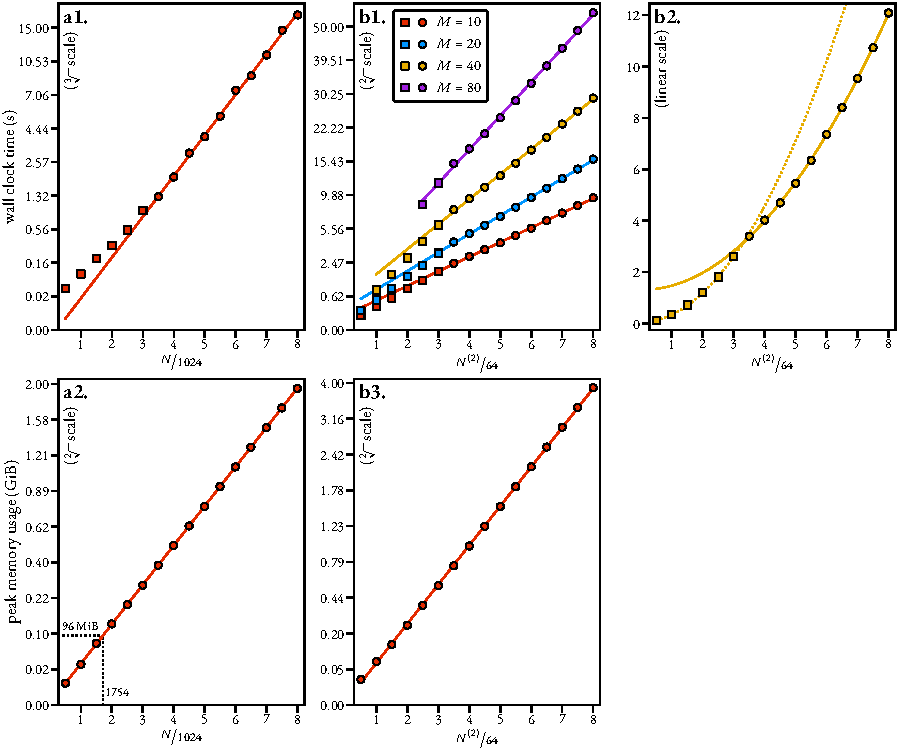
\includegraphics{mpm_profiling/mpm_profiling.pdf}
    \caption[
        Outlines the run times and peak memory consumption of
        the \acs{1D} \acs{MPM} and \acs{2D} \acs{MMEMPM}.
    ]
    {
        Outlines of the run times and peak memory consumption of
        the \acs{1D} \acs{MPM} and \acs{2D} \acs{MMEMPM}.
        The \acp{FID} that were used to acquire these results are described in
        the main text.
        \textbf{a.} panels are related to the \acs{MPM}, while \textbf{b.}
        panels are related to the \acs{MMEMPM}.
        \textbf{a1.} The amount of time required to compute the \ac{MPM}, as a
        function of number of points. Also plotted is a cubic fit of the
        circular points.
        \textbf{a2.} Peak memory consumption in performing the \ac{MPM} as a
        function of the number of points.
        \textbf{b1.} The run times for computing the \ac{MMEMPM} of
        \acp{FID} with $\None = 64$, and variable $\Ntwo$ and $M$.
        \textbf{b2.} The time required to compute the \ac{SVD} of $\EY$ for the
        $M=40$ \acp{FID}. The solid line is a quadratic fit of the circular
        points, while the dashed line is a quadratic fit of the square points.
        \textbf{b3.} Peak memory consumption in performing the \ac{MMEMPM} for
        the $M=40$ \acp{FID}.
    }
    \label{fig:mpm-profiling}
\end{figure}

A series of synthetic \ac{1D} \acp{FID} were constructed, comprising $10$ evenly-spaced
signals, with a
variable number of time-points $N \in \lbrace 512k \hspace*{2pt} \vert
\hspace*{2pt} k \in \lbrace 1, 2, \cdots, 16 \rbrace \rbrace$.
For each \ac{FID}, the \ac{MPM} routine outlined in \cref{lst:mpm} was
performed 5 times, with a pencil parameter $L = \lfloor
\nicefrac{N}{3} \rfloor$.
The mean complete time to run the \ac{MPM} is plotted as a function
of $N$ in panel a1 of \cref{fig:mpm-profiling}, where it can be seen that for
the larger values of $N$ considered, the \ac{MPM} is computed in approximately
$\mathcal{O}({N}^3)$ time. This is because the rate-limiting step of the
\ac{MPM} is the \ac{SVD} of $\Hy$, whose size is to a very good approximation
$\tfrac{2N}{3} \times \tfrac{N}{3}$\footnote{
    \label{fn:svd-complexity}
    The time complexity for the \ac{SVD} of generic a $m \times n$ matrix is
    $\mathcal{O}(\operatorname{min}(m, n)^2 \cdot \operatorname{max}(m, n))$,
    while the space complexity is $\mathcal{O}(mn)$.
}. For smaller values of $N$, a deviation
away from a cubic relationship is observed;
a fit of a cubic function of the form $aN^3 + b$ to the data satisfying $7 \leq k \leq
16$ is plotted in panel a1 to highlight this behaviour.
This arises because the computation of the complex amplitudes using
\cref{eq:complex-amplitudes} has a comparatively significant run time
relative to \ac{SVD} in the low-$N$ regime;
for a $512$ point signal, the \ac{SVD} of $\Hy$ took up roughly 80\% of the
complete run time, while the computation of the complex amplitudes took up
roughly 20\%. For a 8192 point signal, these percentages had changed to
$>\!\!99\%$ and $<\!\!1\%$, respectively.
For all values of $N$,

The \ac{MPM} was run a sixth time on each generated \ac{FID} in order to assess
the effect of $N$ on the space complexity.
The peak \ac{RAM} consumption is plotted in panel a2 of \cref{fig:mpm-profiling}.
A clear quadratic dependence on consumption is realised as function of $N$,
again in agreement with the expected space complexity of the
\ac{SVD}\footnoteref{fn:svd-complexity}.

A similar study was conducted in consideration of the \ac{MMEMPM}. A
series of \ac{2D} \acp{FID} were simulated, all of which all comprised $\None =
64$. The \acp{FID} possessed values of $\Ntwo \in \lbrace 32k
\hspace*{2pt} \vert \hspace*{2pt} \lbrace 1, \cdots, 16 \rbrace \rbrace$.
With the \ac{MPM}, since a
complete \ac{SVD} of the matrix $\Hy$ is computed, the model order is
irrelevant in dictating the run time (at least when $M \ll N$). This is not the
case for the \ac{MMEMPM}; because the \Python implementation used
(\cref{lst:mmempm}) employs a truncated \ac{SVD} in order to compute only the
first $M$ components of $\EY$, the elected model order will have an impact on
run time.  Therefore, \acp{FID} with different model orders were generated: $M
\in \lbrace 10, 20, 40, 80 \rbrace$.

The \ac{MMEMPM} was repeated 5 times for each \ac{FID}, and the mean run
times for each $\Ntwo$ and $M$ considered is plotted in panel b1 of
\cref{fig:mpm-profiling}.
Only the results for cases where the \ac{MMEMPM} was able to yeild a result in
agreement with the data are presented; for certain \acp{FID} with low
$\Ntwo$ and high $M$, appropriate estimation results could not be yielded as
the constituent signals were too poorly resolved.
While in the high-$N$ regime the \ac{MPM} has a cubic time dependence
on the number of points, the \ac{MMEMPM} can be seen to have an approximately
quadratic complexity regarding $\Ntwo$.
For all combinations of $\Ntwo$ and $M$,
the truncated \ac{SVD} was the most time consuming aspect of the routine,
however other steps have notable run times too. Most of the run time is due to
the following five steps (with the relevant lines in \cref{lst:mmempm} given):
\begin{itemize}
    \item Step 1: Construction of $\EY$. This involves building the Hankel matrices
        $\lbrace \symbf{H}_{\symbf{y},\none} : \none \in \lbrace 0, \cdots, 63
        \rbrace \rbrace$, assigning them to the
        correct locations in $\EY$, and finally converting  $\EY$ to a sparse
        matrix\footnote{
            Truncated \ac{SVD} is only available for sparse matrices in
            \textsc{NumPy}\cite{svds}. Some experimenting was done to determine
            the most efficient means of generating $\EY$ in sparse form, and
            subsequently compute its \ac{SVD}.
            It was determined that constructing $\EY$ using a
            standard \textsc{NumPy} array before converting it to
            \ac{CSR} format\cite{csr} was optimal.
        } (Lines \ref{ln:EY-start} to \ref{ln:sparse1}).
    \item Step 2: Truncated \ac{SVD} of $\EY$ to form $\symbf{U}_M$ (Line \ref{ln:sparse2}).
    \item Step 3: Determining $\bdzone$ and  $\symbf{W}^{(1)}$ by computing the
        \ac{EVD} of $\symbf{U}_{M1}^+ \symbf{U}_{M2}^{\vphantom{+}}$ (Lines
        \ref{ln:poles1-start} to \ref{ln:poles1-end}).
    \item Step 4: Generating the second set of signal poles $\bdztwo$, by
        multiplying $\symbf{U}_M$ by the permutation matrix, and extracting
        the diagonal from matrix $\symbf{G}$, computed using \cref{eq:G} (Lines
        \ref{ln:poles2-start} to \ref{ln:poles2-end}). N.B. The \acp{FID} were
        constructed such that the signal poles were unique on all occasions, so
        the additional treatment of repeated signal poles was not necessary.
    \item Step 5: Computation of the complex amplitudes using
        \cref{eq:complex-amplitudes-2d} (Lines \ref{ln:comp-amps-2d-start} to
        \ref{ln:comp-amps-2d-end}).
\end{itemize}
A comparison of the relative times to perform these steps for a few select
pairings of $M$ and $\Ntwo$ is provided by \cref{tab:mmempm-steps}. It can be
seen that as $M$ increases, the relative amount of time spent performing
\ac{SVD} increases, while the amount of time to generate $\EY$ decreases. This
reflects the greater number of iterations required by
the Rayleigh-Ritz method to produce the desired number of \ac{SVD} components,
while the run time to generate $\EY$ remains fixed.

Interestingly, the plots for a given value of $M$ in panel b1 do not exhibit
consistent quadratic behaviour throughout. After a certain value of $\Ntwo$, a
slight reduction in the gradient of the plots in panel b1 can be observed (cf
the square and circular points). This was found to be caused by the \ac{SVD}
computation, whose run times for the $M=40$ \acp{FID} are plotted in panel b2.
The square and circular points both display quadratic behaviour, though the
exact form of the function which
describes them are different ; both sets of points have been fit to curves of
the form of the form $a\Ntwo^2 + b$. After $\Ntwo$ becomes larger than
roughly $200$, the \ac{SVD} run time appears to enter a new regime in which
subsequent increases in  $\Ntwo$ cause the rate of \ac{SVD} to increase at a
slower rate than was the case previously. The exact reason for this probably
lies in the implementation of the Rayleigh-Ritz algorithm, and has not yet been
ascertained.

The peak \ac{RAM} usage for the $M=40$ \acp{FID} as a function of $\Ntwo$ is
plotted in panel b3, where a quadratic complexity is observed. The variation in
memory consumption barely changes as a function of the model order, since the
peak usage is dependent on the size of $\EY$.

It should be noted that the run time and peak \ac{RAM} consumption will also be
(roughly) quadratically dependent on $\None$, just as with $\Ntwo$, i.e.
increasing  $\None$ for  $64$ to  $128$ would cause all the run times in panel
b1 and peak memory usages in panel b3 to quadruple in value.

\begin{table}
    \begin{center}
        \begin{tabular}{ c c c c c c c }
            \toprule
            $\Ntwo$ &
            $M$ &
            Step 1 &
            Step 2 &
            Step 3 &
            Step 4 &
            Step 5 \\
            \midrule
            64 & 10 & 12.2\% & 60.6\% & 2.9\% & 9.7\% & 13.8\% \\
            64 & 40 & 4\% & 74.6\% & 1.9\% & 8.9\% & 9.6\% \\
            512 & 10 & 22.1\% & 67.2\% & 0.2\% & 3.1\% & 7.2\% \\
            512 & 40 & 7.4\% & 81.9\% & 0.1\% & 1.3\% & 9.4\% \\
            512 & 80 & 3.8\% & 85.8\% & 0.1\% & 0.8\% & 9.4\% \\
            \bottomrule
        \end{tabular}
    \end{center}
    \caption[
        A comparison of the relative times to perform the key steps in the \acs{MMEMPM}.
    ]{
        A comparison of the relative times to perform the key steps in the
        \acs{MMEMPM}, for selected pairings on $M$ and $\Ntwo$. See the main
        text for a description of what each step entails.
    }
    \label{tab:mmempm-steps}
\end{table}

\subsection{Computing the Hessian for \acs{NLP}}
